% !TEX program = pdflatex
\documentclass{rapportENSIAS}

\usepackage{longtable}
\usepackage{booktabs}
\usepackage{tabularx}
\usepackage{array}
\usepackage[table]{xcolor}
\usepackage{csquotes}
\usepackage[Glenn]{fncychap}
\usepackage{caption}
\usepackage{indentfirst}
\usepackage{etoolbox}
\captionsetup{hypcap=false}
\graphicspath{{figures/}}

\hypersetup{
    colorlinks=true,
    linkcolor=black,
    filecolor=magenta,
    urlcolor=blue,
    pdftitle={Développement d'un Système de Détection Précoce des AVC par Apprentissage Automatique},
    hypertexnames=false
}

\makeatletter
\pretocmd{\@makechapterhead}{\vspace*{3cm}}{}{}
\makeatother

\renewcommand{\cftchappresnum}{Chapitre\ }
\renewcommand{\cftchapaftersnum}{ :}
\renewcommand{\cftchapnumwidth}{3cm}

\begin{document}
\raggedbottom
\setcounter{secnumdepth}{3}
\setcounter{tocdepth}{3}
\setlength{\parindent}{1cm}

\titre{Développement d'un Système de Détection Précoce des AVC par Apprentissage Automatique}
\UE{Projet de Machine Learning}
\sujet{Spécialisation : Data and Software Sciences}
\enseignant{Pr. IDRI Ali}
\eleves{MOULAY Yasser - GOUMI Soumiya}
\jury{Pr. IDRI Ali}
\dateSoutenance{À compléter}
\anneeUniversitaire{2026 - 2027}

\fairemarges
\fairepagedegarde
\clearpage
\pagenumbering{roman}
\setcounter{page}{1}
\pagestyle{plain}

\chapter*{Remerciements}
\addcontentsline{toc}{chapter}{Remerciements}

Nous adressons nos sincères remerciements au professeur IDRI Ali pour son encadrement, sa disponibilité et la qualité de ses conseils tout au long de ce projet. Son accompagnement et ses retours ont contribué à structurer notre démarche et à mener ce travail avec rigueur.

Nous remercions également l'ensemble du corps professoral de la filière Data and Software Sciences de l'École Nationale Supérieure d'Informatique et d'Analyse des Systèmes (ENSIAS) pour les enseignements et les compétences transmis, qui ont constitué un appui essentiel à la réalisation de ce projet.


\chapter*{Résumé}
\addcontentsline{toc}{chapter}{Résumé}
% Resume a rediger apres validation des resultats finaux.

\clearpage

\chapter*{Abstract}
\addcontentsline{toc}{chapter}{Abstract}
This project investigates the feasibility of an early stroke detection support system using a strongly imbalanced dataset. The original dataset contains 5,110 observations, of which 4.87\% are positive for stroke. Exploratory analysis identifies an association between missing body mass index (BMI) values and observed stroke prevalence: 19.90\% when BMI is missing, compared with 4.26\% when it is available. A dedicated missingness indicator preserves this information without implying a causal relationship.

The preprocessing workflow separates the training and test sets before fitting the imputer and standard scaler. Five model families are compared using stratified cross-validation, with class weighting or SMOTE applied only to training folds. Decision thresholds are then optimized on out-of-fold training probabilities by maximizing the \(F_2\)-score, subject to a minimum specificity of 0.70. The Random Forest is selected according to the pre-established rule based on out-of-fold metrics.

On the independent test set of 1,022 observations, including 50 stroke cases, the selected model, at threshold \(0.5792571442648802\), achieves a recall of 0.80 and a specificity of 0.766. It misses 10 stroke cases and produces 227 false positives, highlighting the trade-off between sensitivity and alert burden. These results are exploratory and do not establish clinical validity; external evaluation and review with healthcare professionals are required before deployment.

\medskip
\noindent\textbf{Keywords:} stroke, imbalanced data, preprocessing, SMOTE, cross-validation, recall, \(F_2\)-score, threshold optimization.

\clearpage

\null
\thispagestyle{plain}
\clearpage

\tableofcontents
\clearpage

\chapter*{Liste des Abréviations}
\addcontentsline{toc}{chapter}{Liste des abréviations}
% La liste des abreviations sera completee pendant la redaction.

\clearpage

\listoffigures
\clearpage
\listoftables
\clearpage

\chapter*{Introduction Générale}
\addcontentsline{toc}{chapter}{Introduction Générale}
\vspace*{-1.1cm}
\begingroup
\footnotesize
\setlength{\parskip}{0.28em}
\setlength{\parindent}{0pt}

\section*{Contexte et motivation}
L'accident vasculaire cérébral (AVC) constitue une urgence médicale dont les conséquences dépendent notamment de la rapidité de la prise en charge. Selon l'Organisation mondiale de la Santé, les estimations pour 2021 recensent 93,8 millions de cas d'AVC et 11,9 millions de nouveaux cas dans le monde ; l'AVC figurait alors parmi les principales causes de décès et d'incapacité \cite{who_stroke_2025}. La prévention et l'orientation rapide des personnes à risque représentent donc des enjeux importants pour les systèmes de santé.

Les données de santé ouvrent des possibilités d'aide à la décision, à condition de distinguer clairement un score statistique d'une conclusion clinique. Le projet \textit{Neuro-Triage} étudie la capacité de modèles d'apprentissage automatique à repérer, parmi des caractéristiques tabulaires telles que l'âge, l'hypertension, les antécédents cardiaques, la glycémie moyenne et l'indice de masse corporelle (IMC), les observations associées à la classe AVC. Le jeu utilisé comprend initialement 5\,110 observations ; la classe positive en représente 4,87\,\%. Ce déséquilibre rend trompeuse une lecture de l'exactitude globale : un classifieur qui prédit systématiquement l'absence d'AVC atteindrait déjà environ 95\,\% d'exactitude, tout en ne détectant aucun cas positif.

\section*{Problématique}
La problématique est donc de construire et d'évaluer un système de priorisation qui ne privilégie pas artificiellement la classe majoritaire. Dans le cadre expérimental retenu, le rappel de la classe AVC est prioritaire, car les faux négatifs correspondent à des cas positifs manqués. Cette priorité doit toutefois être mise en regard de la précision et de la spécificité : un seuil trop bas peut augmenter fortement les alertes erronées et réduire l'utilité opérationnelle du système. Les courbes précision-rappel sont particulièrement informatives dans un contexte de classes rares \cite{saito2015precisionrecall}.

La question de recherche traitée est la suivante : \textit{comment comparer des modèles de classification et choisir un seuil de décision qui améliore le rappel de la classe AVC, tout en contrôlant la spécificité et en limitant les biais d'évaluation ?} Le projet fixe, pour sa sélection expérimentale, un plancher de spécificité de 0,70. Cette valeur est une contrainte méthodologique définie pour l'étude ; elle ne constitue ni une recommandation clinique universelle ni une preuve d'aptitude à un déploiement médical.

\section*{Objectifs et démarche}
Le travail poursuit quatre objectifs :
\begin{itemize}
    \item caractériser la distribution de la cible, les valeurs manquantes et les associations observées dans le jeu de données ;
    \item construire un prétraitement reproductible qui sépare les transformations apprises sur le train de celles appliquées au test, et conserve l'information portée par l'absence d'IMC ;
    \item comparer plusieurs familles de modèles sous validation croisée stratifiée, en plaçant le rééchantillonnage SMOTE dans des pipelines pour éviter qu'il n'affecte les plis de validation ;
    \item optimiser le seuil sur des probabilités hors pli du train à l'aide du score $F_2$, puis réserver le jeu de test à l'évaluation finale.
\end{itemize}

Le choix du score $F_2$ traduit, dans le protocole, une importance plus élevée accordée au rappel qu'à la précision. Il ne supprime pas pour autant le compromis entre faux négatifs et faux positifs : la sélection des modèles est également soumise au plancher de spécificité défini précédemment. La régression logistique pondérée est conservée comme référence interprétable, à côté de modèles d'ensemble régularisés.

Il convient enfin de préciser la portée du résultat attendu. Le jeu de données comporte une étiquette binaire « stroke », mais ne documente pas à lui seul un protocole prospectif ni l'instant auquel les variables ont été recueillies par rapport à l'apparition des symptômes. L'étude mesure donc une performance de classification sur ce jeu et ne démontre pas une détection pré-symptomatique. Le modèle produit un score expérimental d'aide à la priorisation ; il ne remplace ni l'évaluation clinique ni les examens diagnostiques.

\section*{Organisation du rapport}
Le rapport est organisé en quatre chapitres. Le premier présente le jeu de données et les résultats de l'analyse exploratoire. Le deuxième détaille le prétraitement et les mesures de prévention de la fuite de données. Le troisième expose le protocole de modélisation, le benchmark et la validation croisée. Le quatrième présente l'optimisation du seuil, l'évaluation sur le jeu de test et les limites de l'étude. Une conclusion générale synthétise les résultats et les perspectives.
\endgroup


\clearpage
\pagenumbering{arabic}
\chapter{Compréhension et exploration des données}
\label{chap:eda}
\thispagestyle{plain}

\section{Objectifs de l'exploration}
Cette première étape vise à comprendre la structure du jeu de données, la distribution de la variable cible et les relations descriptives entre les variables candidates et la présence d'un AVC. L'exploration sert à formuler des hypothèses et à orienter les choix de préparation et d'évaluation ; elle ne permet, à elle seule, ni d'établir une causalité ni de valider un outil clinique.

\section{Présentation du jeu de données}
Le fichier brut contient \textbf{5\,110 observations et 12 colonnes}. La cible binaire \texttt{stroke} indique si un AVC est enregistré pour l'observation considérée (\texttt{stroke=1}) ou non (\texttt{stroke=0}). Les variables explicatives couvrent l'âge, l'hypertension, les antécédents de maladie cardiaque, le niveau moyen de glucose, l'indice de masse corporelle (IMC), ainsi que des caractéristiques démographiques et comportementales.

\begin{table}[H]
    \centering
    \caption{Nature des variables du jeu de données initial}
    \label{tab:eda-variable-types}
    \renewcommand{\arraystretch}{1.2}
    \begin{tabularx}{\textwidth}{@{}>{\raggedright\arraybackslash}p{3.1cm}X@{}}
        \toprule
        \textbf{Type} & \textbf{Variables}\\
        \midrule
        Identifiant & \texttt{id} (identifiant de ligne, non destiné à être utilisé comme prédicteur)\\
        Numérique & \texttt{age}, \texttt{avg\_glucose\_level}, \texttt{bmi}\\
        Binaire & \texttt{hypertension}, \texttt{heart\_disease}\\
        Catégoriel & \texttt{gender}, \texttt{ever\_married}, \texttt{work\_type}, \texttt{Residence\_type}, \texttt{smoking\_status}\\
        Cible & \texttt{stroke} (0 : aucun AVC enregistré ; 1 : AVC enregistré)\\
        \bottomrule
    \end{tabularx}
\end{table}

Le jeu brut ne comporte ni doublon de ligne ni doublon d'identifiant. La colonne \texttt{id} est donc utile pour l'identification des enregistrements, mais ne porte pas de caractéristique clinique pertinente et sera écartée des variables d'entrée. L'exploration relève également une modalité \texttt{Other} pour le genre, représentée par une seule observation ; son traitement est documenté dans l'étape de préparation afin d'éviter qu'une modalité quasi isolée ne perturbe l'encodage.

\section{Déséquilibre de la variable cible}
La distribution de \texttt{stroke}, représentée à la figure~\ref{fig:target_dist}, met en évidence une forte rareté des cas positifs.

\begin{table}[H]
    \centering
    \caption{Répartition de la cible dans le jeu brut}
    \label{tab:eda-target-distribution}
    \begin{tabular}{@{}lrr@{}}
        \toprule
        \textbf{Classe} & \textbf{Effectif} & \textbf{Proportion}\\
        \midrule
        \texttt{stroke=0} & 4\,861 & 95,13\,\%\\
        \texttt{stroke=1} & 249 & 4,87\,\%\\
        \bottomrule
    \end{tabular}
\end{table}

\begin{figure}[H]
    \centering
    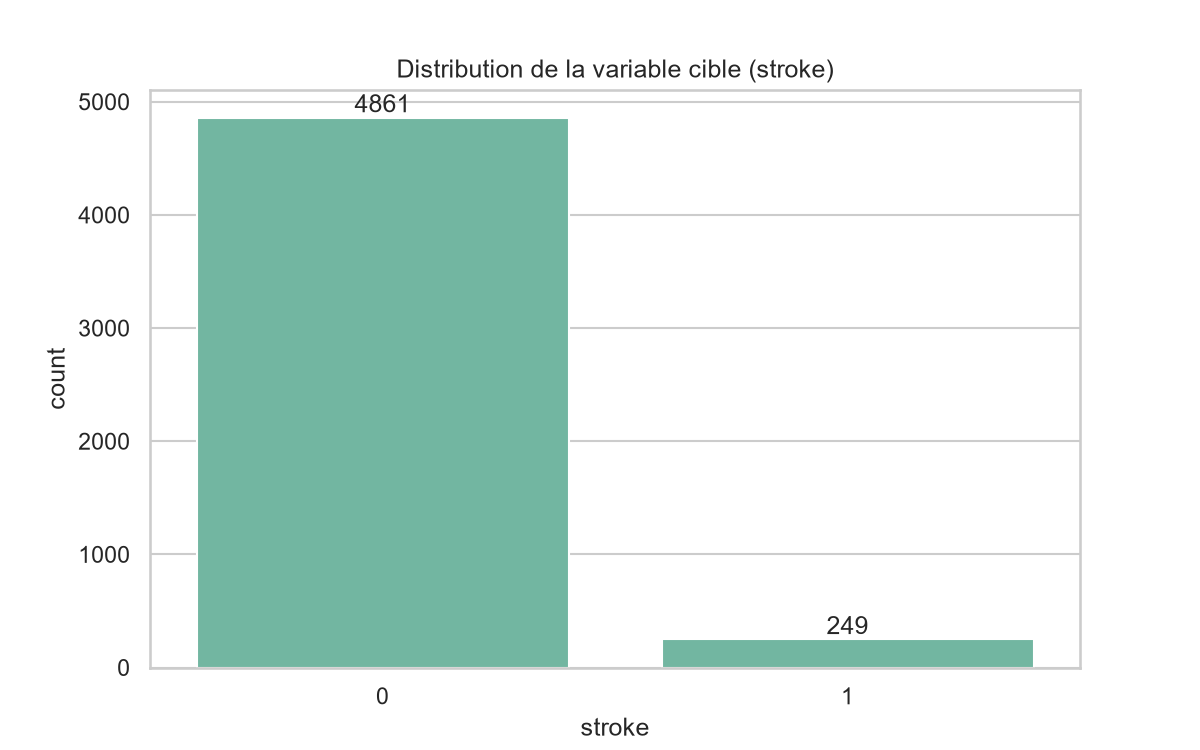
\includegraphics[width=0.72\textwidth]{02_target_distribution.png}
    \caption{Distribution de la variable cible \texttt{stroke}}
    \label{fig:target_dist}
\end{figure}

Cette asymétrie conditionne la suite du projet. Un modèle qui attribuerait la classe majoritaire à toutes les observations afficherait déjà environ 95\,\% d'exactitude, tout en manquant les 249 cas positifs. L'exactitude ne peut donc pas servir seule de critère de sélection. Le benchmark devra examiner spécifiquement le rappel de la classe AVC, la précision, la spécificité et des métriques adaptées aux classes déséquilibrées, notamment la PR-AUC. La stratégie de modélisation intégrera également une pondération des classes ou un rééchantillonnage réalisé uniquement dans les plis d'entraînement.

\section{Variables numériques et tests de Mann--Whitney}
\subsection{Forme des distributions}
Les distributions numériques présentées à la figure~\ref{fig:eda-numeric-distributions} montrent des formes différentes selon la variable. L'âge est relativement peu asymétrique (skewness de $-0{,}14$), tandis que le niveau moyen de glucose et l'IMC présentent une asymétrie à droite (respectivement $1{,}57$ et $1{,}06$). Une comparaison fondée exclusivement sur les moyennes ou sur une hypothèse de normalité serait donc insuffisante pour caractériser les écarts entre groupes.

\begin{figure}[H]
    \centering
    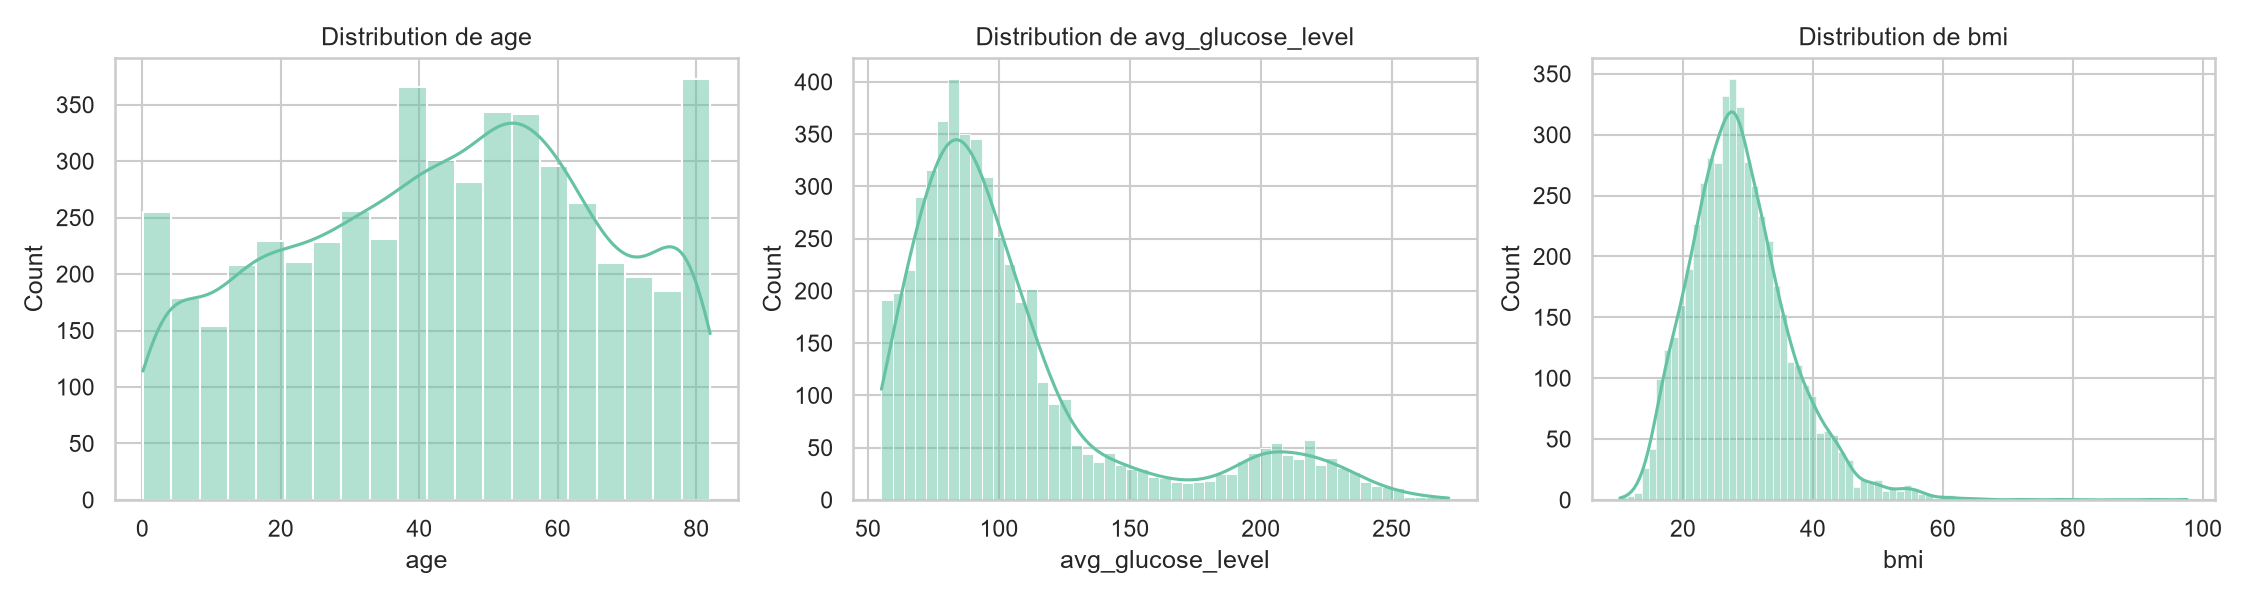
\includegraphics[width=0.92\textwidth]{03_num_distributions.png}
    \caption{Distributions des variables numériques dans le jeu brut}
    \label{fig:eda-numeric-distributions}
\end{figure}

\subsection{Comparaison exploratoire des groupes}
Pour comparer les observations des classes \texttt{stroke=0} et \texttt{stroke=1}, le notebook applique le test non paramétrique de Mann--Whitney à l'âge, au niveau moyen de glucose et à l'IMC. Ce test, fondé sur les rangs, permet de rechercher une différence de distribution sans imposer une loi normale aux mesures. Le tableau~\ref{tab:eda-mann-whitney} présente, à titre descriptif, les moyennes calculées pour chaque classe et les valeurs $p$ obtenues.

\begin{table}[H]
    \centering
    \caption{Comparaison des variables numériques selon la cible}
    \label{tab:eda-mann-whitney}
    \renewcommand{\arraystretch}{1.15}
    \begin{tabular}{@{}lrrr@{}}
        \toprule
        \textbf{Variable} & \textbf{Moyenne, classe 0} & \textbf{Moyenne, classe 1} & \textbf{Valeur $p$}\\
        \midrule
        \texttt{age} & 41,97 & 67,73 & $3{,}73 \times 10^{-71}$\\
        \texttt{avg\_glucose\_level} & 104,80 & 132,54 & $3{,}64 \times 10^{-9}$\\
        \texttt{bmi} & 28,82 & 30,47 & $1{,}03 \times 10^{-4}$\\
        \bottomrule
    \end{tabular}
\end{table}

Les trois valeurs $p$ sont très inférieures au seuil exploratoire de 0,05 : les distributions observées diffèrent donc entre les groupes dans cet échantillon. L'âge présente l'écart de moyenne le plus marqué, suivi du niveau moyen de glucose ; l'écart de moyenne d'IMC est plus limité, mais le test détecte également une différence de rangs. Ces résultats ne démontrent ni un lien causal ni une capacité de prédiction indépendante : ils ne tiennent pas compte des interactions entre variables et doivent être interprétés en tenant compte du déséquilibre de la cible et des données manquantes. Les courbes de densité de la figure~\ref{fig:eda-numeric-by-stroke} complètent cette comparaison visuelle.

\begin{figure}[H]
    \centering
    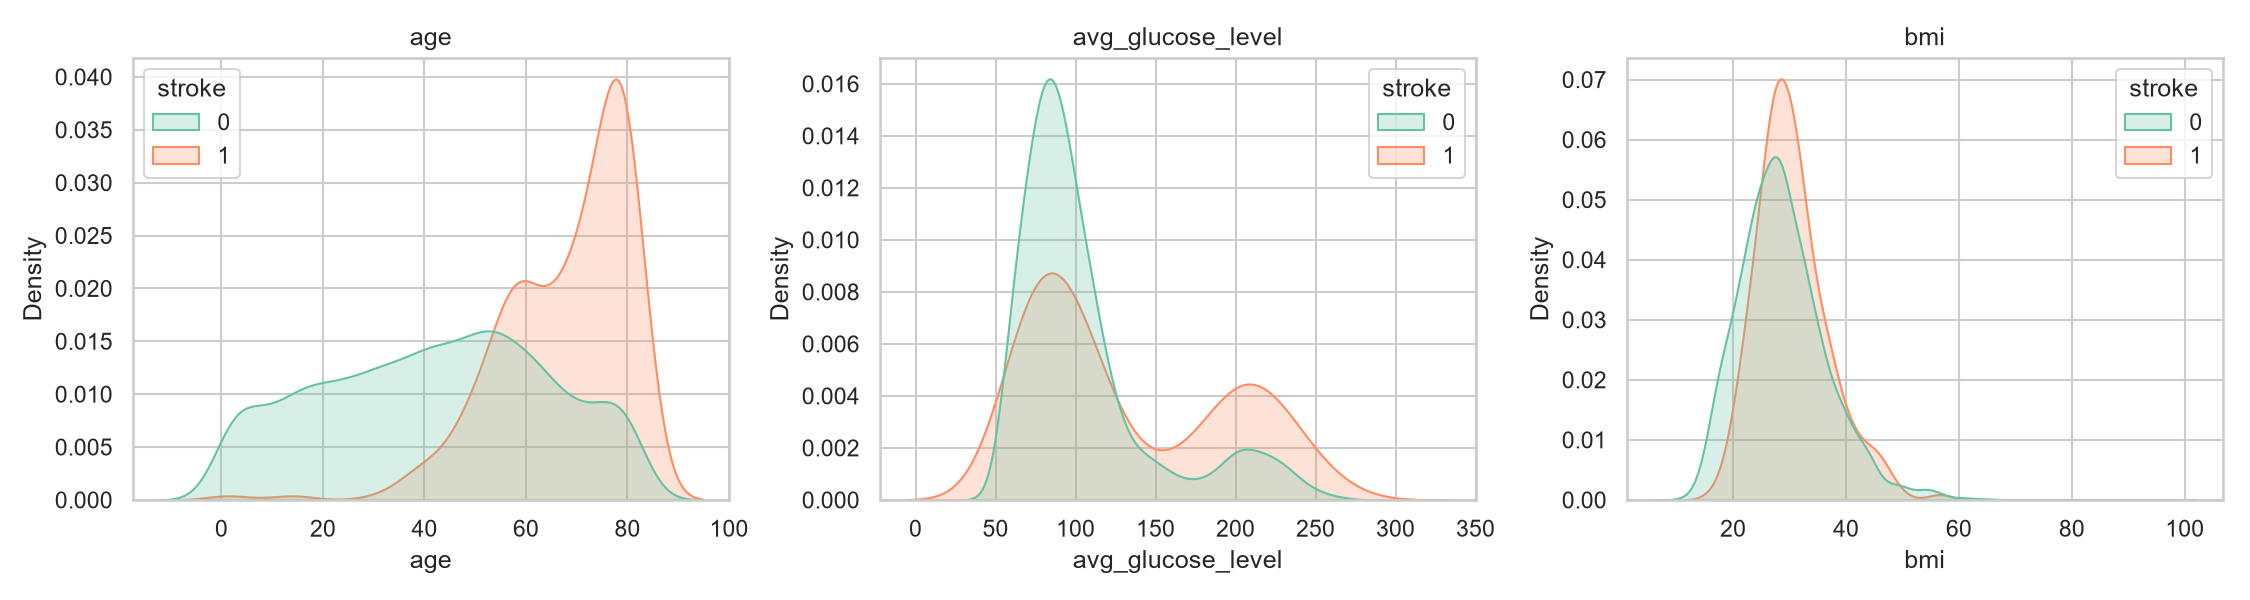
\includegraphics[width=0.92\textwidth]{05_num_kde_by_stroke.png}
    \caption{Distributions des variables numériques par classe de \texttt{stroke}}
    \label{fig:eda-numeric-by-stroke}
\end{figure}

\section{Valeurs manquantes de l'IMC : un signal à préserver}
La seule variable présentant des valeurs manquantes dans l'exploration est l'IMC : \textbf{201 valeurs, soit 3,93\,\%} des observations. Leur répartition selon la cible est particulièrement informative :

\begin{table}[H]
    \centering
    \caption{Prévalence observée de la classe AVC selon la disponibilité de l'IMC}
    \label{tab:eda-bmi-missing}
    \renewcommand{\arraystretch}{1.15}
    \begin{tabular}{@{}lrrr@{}}
        \toprule
        \textbf{Disponibilité de l'IMC} & \textbf{Effectif} & \textbf{Part du jeu} & \textbf{Taux de \texttt{stroke=1}}\\
        \midrule
        IMC renseigné & 4\,909 & 96,07\,\% & 4,26\,\%\\
        IMC manquant & 201 & 3,93\,\% & \textbf{19,90\,\%}\\
        \bottomrule
    \end{tabular}
\end{table}

Le taux d'AVC parmi les observations sans IMC est donc supérieur de 15,64 points de pourcentage au taux observé lorsque l'IMC est renseigné. Dans le cadre de ce jeu, ce contraste contredit la plausibilité d'une hypothèse stricte de données manquantes complètement au hasard (MCAR), selon laquelle l'absence de mesure serait indépendante des variables observées et non observées \cite{rubin1976missing}. Il s'agit d'un constat descriptif : il ne permet pas, à lui seul, d'identifier le mécanisme de non-réponse ni de distinguer un mécanisme MAR d'un mécanisme MNAR. Une analyse causale de la raison de l'absence de mesure demanderait des informations supplémentaires sur le processus de collecte.

Imputer directement les valeurs manquantes par une médiane ferait disparaître le fait qu'une mesure était absente. Pour éviter cette perte d'information, la préparation crée donc une variable indicatrice binaire \texttt{bmi\_missing} avant l'imputation : elle vaut 1 lorsque l'IMC initial est manquant et 0 autrement. L'IMC lui-même est ensuite imputé par la médiane estimée sur le jeu d'entraînement seulement (28,10 dans l'exécution documentée). Cette stratégie conserve un signal potentiellement utile sans prétendre que l'absence d'IMC cause l'AVC ; son apport devra être évalué hors échantillon et contrôlé contre le risque d'apprendre un biais propre au processus de collecte.

\section{Variables catégorielles, âge et valeurs atypiques}
\subsection{Associations observées pour les variables catégorielles}
Le notebook utilise des tests du $\chi^2$ sur les tableaux de contingence entre la cible et les variables catégorielles ou binaires. Les associations les plus marquées dans l'échantillon concernent les antécédents de maladie cardiaque ($p=2{,}09 \times 10^{-21}$), l'hypertension ($p=1{,}66 \times 10^{-19}$), le statut marital ($p=1{,}64 \times 10^{-14}$), le type d'emploi ($p=5{,}40 \times 10^{-10}$) et le statut tabagique ($p=2{,}09 \times 10^{-6}$). En revanche, les tests ne mettent pas en évidence d'association statistiquement significative pour le type de résidence ($p=0{,}298$) ni pour le genre ($p=0{,}790$). Ces tests restent exploratoires et ne prouvent pas de relation causale ; la modalité de genre représentée par une seule ligne invite en particulier à interpréter le résultat correspondant avec prudence.

\subsection{Gradient descriptif selon l'âge}
Le taux d'AVC observé augmente avec les tranches d'âge : il est de 0,22\,\% avant 18 ans, 0,45\,\% entre 18 et 40 ans, 4,10\,\% entre 40 et 60 ans, 12,96\,\% entre 60 et 80 ans et 19,83\,\% au-delà de 80 ans. Cette évolution descriptive concorde avec l'écart observé lors du test de Mann--Whitney, sans isoler l'effet propre de l'âge des autres facteurs associés.

\begin{figure}[H]
    \centering
    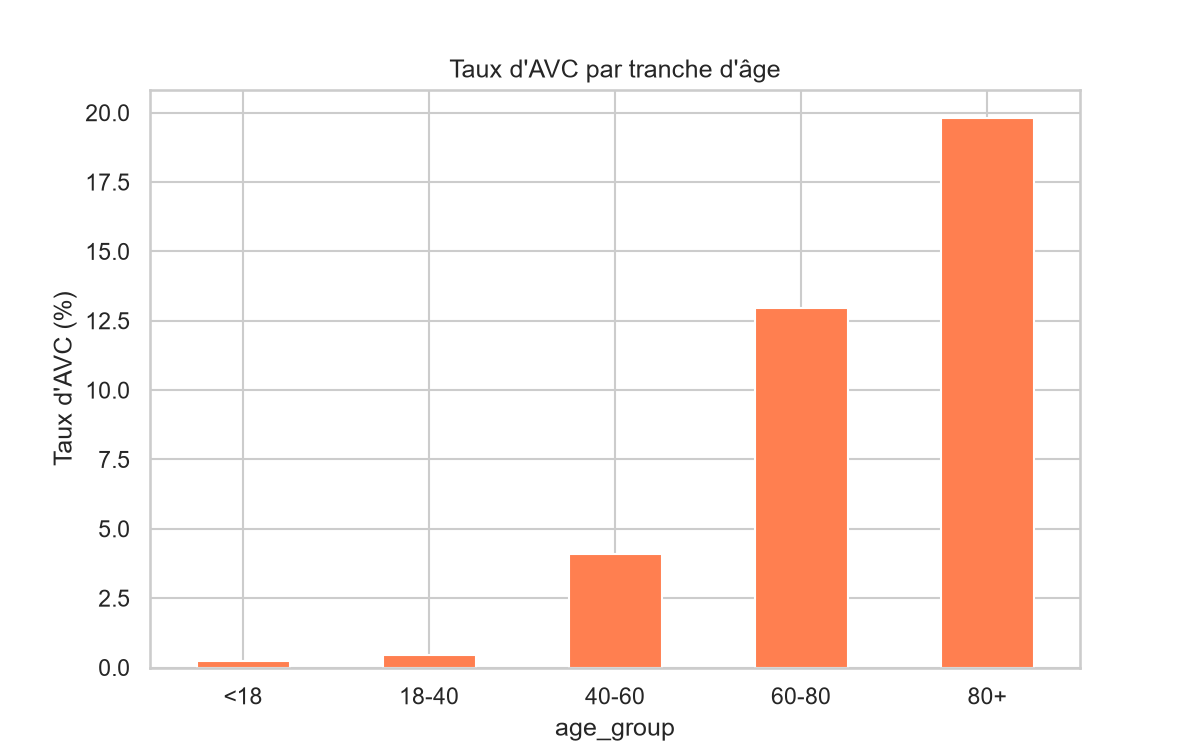
\includegraphics[width=0.78\textwidth]{06_stroke_rate_by_age.png}
    \caption{Taux d'AVC observé par tranche d'âge}
    \label{fig:eda-stroke-by-age}
\end{figure}

\subsection{Valeurs extrêmes et statut tabagique « Unknown »}
La règle de l'écart interquartile signale 627 valeurs extrêmes de glycémie moyenne (12,3\,\%) et 110 valeurs d'IMC (2,2\,\%). L'IMC maximal atteint 97,6, alors que la borne supérieure calculée par la règle IQR est de 47,5. Ces constats motivent un contrôle de l'influence des valeurs extrêmes ; le prétraitement retient un plafonnement de l'IMC à 60 plutôt qu'une suppression massive des lignes, afin de limiter l'effet des extrêmes tout en conservant les observations.

La modalité \texttt{Unknown} du statut tabagique concerne 1\,544 observations et est fortement représentée chez les jeunes (âge médian de 23 ans). Dans le prétraitement, 614 observations ayant un âge inférieur à 15 ans et un statut \texttt{Unknown} sont recodées en \texttt{never smoked}. Cette règle vise à éviter que l'absence de renseignement, attendue dans cette tranche d'âge, soit apprise comme une catégorie clinique équivalente chez les enfants. Elle constitue néanmoins une hypothèse de préparation, et non une observation vérifiée du comportement tabagique ; son effet doit être interprété avec prudence.

\section{Synthèse et implications pour la suite}
L'EDA met en évidence trois contraintes structurantes : la faible prévalence de la classe AVC, les différences de distributions entre les classes et l'association marquée entre l'absence d'IMC et la cible. Ces constats motivent l'emploi de métriques sensibles à la classe positive, la conservation de l'indicateur \texttt{bmi\_missing} et une préparation qui distingue les transformations déterminées a priori de celles apprises sur le train. Le chapitre suivant détaille le split des données, l'imputation et la standardisation, ainsi que les règles de nettoyage retenues.

\chapter{Prétraitement des données et ingénierie des caractéristiques}
\label{chap:preprocessing}
\thispagestyle{plain}

\section{Principes et séquence de préparation}
Le prétraitement transforme les enregistrements bruts en une matrice numérique compatible avec les algorithmes de classification. Pour préserver la validité de l'évaluation, les opérations doivent être séparées selon leur nature : les règles déterministes de nettoyage et d'ingénierie sont documentées, tandis que les paramètres appris à partir de la distribution des données sont ajustés uniquement sur le jeu d'entraînement.

La séquence appliquée est la suivante : retrait de l'identifiant, nettoyage des modalités rares et transformations explicites, création des variables indicatrices, séparation stratifiée train/test, puis ajustement de l'imputation et de la standardisation sur le train. Le jeu de test ne sert ensuite qu'à appliquer les transformations déjà ajustées et à évaluer les modèles.

\section{Nettoyage et ingénierie des caractéristiques}
\subsection{Conservation du signal associé à l'IMC manquant}
Comme l'a montré le chapitre~\ref{chap:eda}, l'absence d'IMC est associée à un taux de \texttt{stroke=1} de 19,90\,\%, contre 4,26\,\% lorsque l'IMC est renseigné (tableau~\ref{tab:eda-bmi-missing}). Remplacer directement les valeurs absentes par une valeur centrale ferait perdre cette information de disponibilité.

Le notebook crée donc la variable binaire \texttt{bmi\_missing} \textbf{avant l'imputation} :
\[
\texttt{bmi\_missing}_i =
\begin{cases}
1 & \text{si l'IMC de l'observation } i \text{ est manquant},\\
0 & \text{sinon.}
\end{cases}
\]
L'IMC et son indicateur sont ainsi deux caractéristiques distinctes : la première contient la mesure imputée, tandis que la seconde signale qu'elle n'a pas été observée initialement. Cette représentation conserve un signal prédictif potentiel sans attribuer de causalité à la non-réponse et sans remplacer l'information manquante par un indicateur clinique inventé.

\subsection{Valeurs extrêmes et plafonnement de l'IMC}
L'EDA a relevé un IMC maximal de 97,6, au-delà de la borne supérieure de 47,5 obtenue par la règle de l'écart interquartile. Le prétraitement plafonne les valeurs d'IMC à 60 :
\[
\texttt{bmi}_{i}^{\,\mathrm{cap}} = \min(\texttt{bmi}_{i}, 60).
\]
Le seuil est appliqué comme une règle fixe, sans calculer de paramètre à partir du jeu de test. Le choix du plafonnement plutôt que de la suppression des lignes vise à limiter l'influence de valeurs extrêmes tout en conservant les autres informations du même patient. Cette conservation est importante dans un jeu où des variables telles que la glycémie moyenne diffèrent entre les classes (tableau~\ref{tab:eda-mann-whitney}) : supprimer une ligne sur le seul critère de l'IMC éliminerait également ces mesures et les antécédents associés. Le plafonnement ne prétend pas déterminer la validité clinique d'une valeur ; il réduit seulement son poids numérique dans les transformations ultérieures.

\subsection{Nettoyage des modalités et encodage}
La colonne \texttt{id} est retirée des prédicteurs, car elle identifie les enregistrements sans représenter un attribut clinique. L'unique observation portant la modalité \texttt{Other} dans \texttt{gender} est écartée dans le notebook de préparation, faute d'effectif suffisant pour estimer ou exploiter cette modalité dans ce jeu.

Les variables binaires sont converties au moyen de correspondances explicites : \texttt{gender} (Female/Male), \texttt{ever\_married} (No/Yes) et \texttt{Residence\_type} (Rural/Urban). Les variables \texttt{work\_type} et \texttt{smoking\_status} sont développées avec un One-Hot Encoding au moyen de \texttt{pandas.get\_dummies}, avec \texttt{drop\_first=True}. La catégorie de référence omise évite une dépendance linéaire exacte entre toutes les colonnes d'une même variable catégorielle, notamment pour la régression logistique. Les colonnes binaires produites sont stockées sous forme d'entiers 0/1.

Cette expansion est déterministe et n'utilise pas la cible. Dans le notebook, elle est effectuée avant le split pour établir une matrice de colonnes commune aux deux sous-ensembles. Cette étape consulte donc le support des modalités des variables explicatives de l'ensemble du jeu, même si elle n'en estime ni moyenne ni médiane. Pour une isolation stricte du schéma de catégories en production, une évolution recommandée consiste à ajuster un \texttt{OneHotEncoder(handle\_unknown="ignore")} sur le train uniquement, puis à sérialiser l'encodeur avec les autres transformations. Dans la version actuelle, l'ordre final des colonnes est figé dans les métadonnées et doit être respecté par l'API.

\section{Séparation train/test et prévention de la fuite de données}
\subsection{Split stratifié avant les transformations apprises}
Après le retrait de l'unique ligne \texttt{gender=Other}, le jeu contient 5\,109 observations. La séparation est réalisée avec \texttt{train\_test\_split}, un rapport 80/20, \texttt{stratify=y} et la graine aléatoire 42. Elle produit 4\,087 observations d'entraînement et 1\,022 de test. La proportion de la classe AVC reste proche dans les deux ensembles : 4,87\,\% dans le train et 4,89\,\% dans le test.

\textbf{Le split précède l'imputation et la standardisation.} C'est une contrainte essentielle : le jeu de test doit rester une approximation indépendante de données futures, et ne doit pas contribuer à l'estimation des paramètres qui seront ensuite évalués sur lui.

\subsection{Pourquoi les statistiques globales créeraient une fuite}
Soit \(X_{\mathrm{train}}\) le jeu d'entraînement et \(X_{\mathrm{test}}\) le jeu réservé à l'évaluation. La médiane d'imputation doit être estimée à partir du train :
\[
\widehat{m}_{\mathrm{train}}
= \operatorname{median}\!\left(X_{\mathrm{train}}^{\mathrm{IMC}}\right).
\]
De même, pour chaque variable numérique \(j\), la standardisation utilise uniquement la moyenne et l'écart-type du train :
\[
\widehat{\mu}_{j,\mathrm{train}}
= \frac{1}{n_{\mathrm{train}}}\sum_{i \in \mathrm{train}} x_{ij},
\qquad
\widehat{\sigma}_{j,\mathrm{train}}
= \sqrt{\frac{1}{n_{\mathrm{train}}}\sum_{i \in \mathrm{train}}
(x_{ij}-\widehat{\mu}_{j,\mathrm{train}})^2}.
\]
Les valeurs du train sont alors transformées par
\[
z_{ij}^{\mathrm{train}}
= \frac{x_{ij}-\widehat{\mu}_{j,\mathrm{train}}}
       {\widehat{\sigma}_{j,\mathrm{train}}},
\]
et les observations de test par les \emph{mêmes} paramètres estimés sur le train. Le jeu de test ne sert jamais à recalculer une médiane, une moyenne ou une dispersion.

À l'inverse, calculer une médiane ou une moyenne sur \(X_{\mathrm{train}}\cup X_{\mathrm{test}}\) rendrait les transformations dépendantes de la distribution du jeu de test. Même sans utiliser explicitement ses étiquettes, le protocole aurait déjà incorporé des informations sur les observations réservées à l'évaluation. La mesure finale ne représenterait donc plus une évaluation strictement indépendante et pourrait être artificiellement optimiste ou déplacée selon la distribution du test.

\subsection{Ajustement de l'imputeur et du scaler}
L'imputeur \texttt{SimpleImputer(strategy="median")} est ajusté sur la colonne \texttt{bmi} du train ; sa médiane estimée est 28,10. La méthode \texttt{transform} applique ensuite cette valeur au train et au test, sans réajustement sur ce dernier. Le contrôle du notebook confirme qu'il ne subsiste aucune valeur manquante après transformation.

Le \texttt{StandardScaler} est ajusté uniquement sur \texttt{age}, \texttt{avg\_glucose\_level} et \texttt{bmi} du train, puis appliqué au test avec les paramètres enregistrés. Les variables binaires, les indicateurs et les colonnes One-Hot ne sont pas standardisés. Ce traitement limite les écarts d'échelle pour les algorithmes sensibles aux distances ou aux amplitudes numériques, sans laisser le jeu de test influer sur les statistiques de centrage et de réduction.

\section{Persistance des transformations et contrat de l'API}
Pour que l'inférence reproduise le traitement de l'entraînement, le notebook sauvegarde l'imputeur et le scaler ajustés dans \texttt{bmi\_imputer.joblib} et \texttt{scaler.joblib}. Le fichier \texttt{preprocessing\_metadata.json} documente notamment la cible, les correspondances binaires, la liste ordonnée des colonnes finales, les variables numériques, le plafond d'IMC et le nom de l'indicateur de données manquantes.

L'ordre des caractéristiques constitue un contrat d'interface : un même vecteur numérique placé dans une colonne différente n'a plus la même signification pour le modèle. La liste \texttt{feature\_columns} doit donc être utilisée pour ordonner les entrées de l'API avant l'appel au modèle. De même, l'API doit réutiliser les correspondances catégorielles et les objets d'imputation et de standardisation sauvegardés ; elle ne doit jamais réestimer ces transformations à partir d'une requête ou d'un lot de nouveaux patients.

Dans une architecture FastAPI, ces fichiers doivent être versionnés avec le modèle correspondant, chargés depuis un emplacement contrôlé et remplacés de manière atomique lors d'une nouvelle mise à jour. Les artefacts \texttt{joblib} ne doivent être chargés que depuis une source de confiance. Enfin, les données de santé transmises à l'API et les journaux applicatifs doivent suivre les règles de contrôle d'accès, de minimisation et de protection des données du projet ; les identifiants directs ne sont pas des caractéristiques du modèle et ne doivent pas être réintroduits dans les vecteurs d'inférence.

\section{Synthèse}
Le protocole sépare explicitement les règles fixes de préparation des statistiques apprises. Il conserve l'information de non-réponse de l'IMC, limite l'influence des valeurs extrêmes sans éliminer les autres caractéristiques des patients et fige les transformations dépendantes de la distribution en les ajustant exclusivement sur le train. La sérialisation des paramètres et de l'ordre des colonnes fournit enfin un contrat reproductible entre l'entraînement et l'API, sous réserve de compléter le schéma One-Hot par une politique explicite de gestion des catégories inconnues avant toute mise en production.

% Chapitre 3 : benchmark, validation croisee et selection des modeles.

\chapter{Évaluation finale et optimisation du seuil}
\label{chap:evaluation}
\thispagestyle{plain}

\section{Du score probabiliste à la décision clinique}
Un classifieur binaire ne fournit pas directement une décision médicale : il estime d'abord un score ou une probabilité d'appartenance à la classe positive, puis un seuil transforme ce score en prédiction. Avec le seuil conventionnel de 0,50, une observation est déclarée positive si sa probabilité estimée atteint au moins 0,50. Cette convention ne tient pas compte, à elle seule, du déséquilibre de la cible ni du coût asymétrique des erreurs dans un contexte de dépistage.

Lorsque les AVC sont rares et que les faux négatifs sont particulièrement coûteux, un seuil non validé peut laisser trop de cas positifs sous la limite de décision. Le seuil 0,50 n'est cependant pas nécessairement trop élevé pour tous les modèles : son effet dépend de la distribution et de la calibration des probabilités. Il doit donc être choisi empiriquement sur les données d'entraînement, selon un objectif explicite, et non abaissé arbitrairement. Dans l'exécution documentée ici, les seuils optimaux sont même supérieurs à 0,50 ; le seuil de 0,18 donné comme exemple ne correspond pas aux résultats du notebook.

\section{Recherche du seuil sur les probabilités hors pli}
\subsection{Prédictions out-of-fold}
Pour chaque finaliste — régression logistique pondérée, Random Forest pondérée et XGBoost avec \texttt{scale\_pos\_weight} — les probabilités de la classe AVC sont estimées sur le jeu d'entraînement au moyen de \texttt{cross\_val\_predict(method="predict\_proba")}, avec une validation croisée \texttt{StratifiedKFold} à cinq plis. Ainsi, chaque observation d'entraînement reçoit une probabilité produite par un modèle qui n'a pas été ajusté sur cette observation. Le seuil est donc déterminé à partir de prédictions hors pli, plutôt qu'à partir des probabilités d'ajustement du modèle entraîné sur toutes les données, ce qui limite un seuil artificiellement optimiste.

À partir des probabilités hors pli, la courbe précision-rappel fournit, pour chaque seuil candidat, une précision \(P\) et un rappel \(R\). Le score \(F_\beta\) est une moyenne harmonique pondérée de ces deux mesures. Le choix \(\beta=2\) donne davantage de poids au rappel qu'à la précision :
\[
F_2 = (1+\beta^2)\frac{P\,R}{\beta^2P+R}
    = \frac{5\,P\,R}{4P+R}.
\]
Le seuil retenu pour chaque modèle est celui qui maximise le \(F_2\) calculé sur ces probabilités hors pli. Les divisions par zéro sont traitées dans le calcul numérique afin que les seuils sans prédictions positives ne provoquent pas d'échec. La figure~\ref{fig:threshold-f2} présente les courbes obtenues et les seuils maximisants.

\begin{figure}[H]
    \centering
    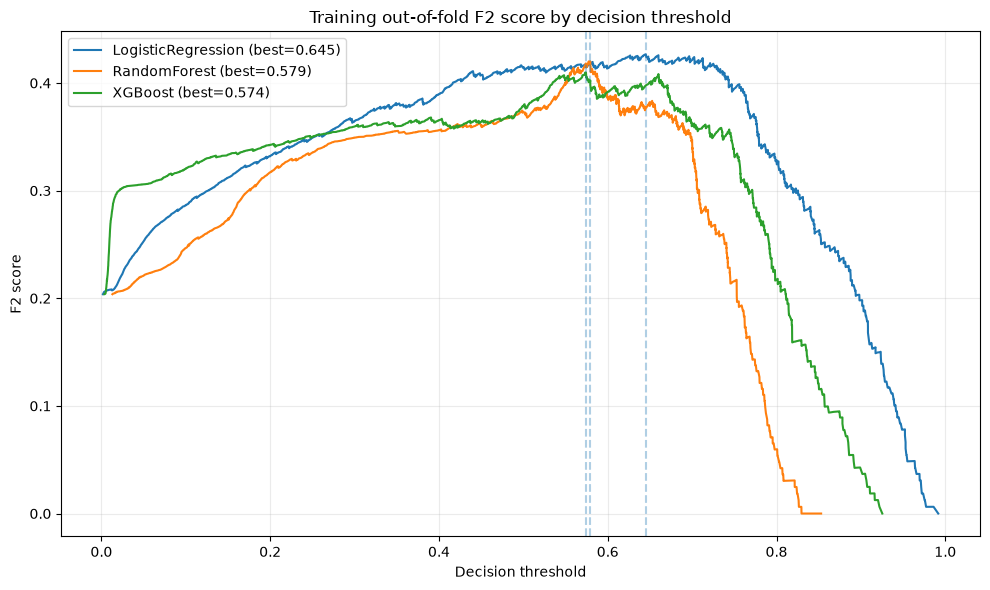
\includegraphics[width=0.82\textwidth]{figures/04_threshold_f2.png}
    \caption{Score \(F_2\) selon le seuil, calculé sur les probabilités out-of-fold du jeu d'entraînement. Les lignes verticales indiquent les seuils maximisant le \(F_2\) pour chaque modèle.}
    \label{fig:threshold-f2}
\end{figure}

Les seuils et scores hors pli effectivement obtenus sont synthétisés au tableau~\ref{tab:threshold-oof}. Ces valeurs sont des résultats d'optimisation sur le train, et non des mesures obtenues sur le test.

\begin{table}[H]
    \centering
    \caption{Optimisation des seuils sur les prédictions out-of-fold du train}
    \label{tab:threshold-oof}
    \small
    \begin{tabular}{@{}lrrr@{}}
        \toprule
        \textbf{Modèle} & \textbf{Seuil optimal} & \textbf{\(F_2\) OOF} & \textbf{Rappel OOF}\\
        \midrule
        LogisticRegression & 0,645058 & 0,427 & 0,678\\
        RandomForest & 0,579257 & 0,420 & 0,769\\
        XGBoost & 0,574196 & 0,410 & 0,729\\
        \bottomrule
    \end{tabular}
\end{table}

\subsection{Plancher de spécificité et compromis d'alertes}
Maximiser le rappel sans contrainte peut conduire à classer un grand nombre de patients non AVC comme positifs. La spécificité mesure la proportion de négatifs correctement rejetés :
\[
\operatorname{Specificite} = \frac{TN}{TN+FP},
\]
où \(TN\) et \(FP\) désignent respectivement les vrais négatifs et les faux positifs. Pour rendre explicite le compromis avec la charge d'alertes, un plancher de spécificité de 0,70 a été fixé avant l'examen des résultats du test. Il limite à 30\,\% au plus le taux de faux positifs parmi les sujets sains, selon le critère retenu par le protocole.

Ce seuil de 0,70 est une contrainte opérationnelle de cette étude, et non une norme clinique universelle. Il sert à éviter une stratégie qui maximiserait le rappel au prix d'un nombre d'alertes potentiellement ingérable, mais sa pertinence doit être confirmée avec les professionnels de santé et le contexte réel de déploiement. La sélection du modèle est effectuée exclusivement à partir des métriques OOF : parmi les candidats dont la spécificité OOF atteint le plancher, la règle retient celui qui présente le rappel OOF le plus élevé, avec le \(F_2\) et la spécificité comme critères de départage.

\section{Évaluation finale sur le test indépendant}
Une fois les seuils déterminés et la règle de sélection arrêtée sur le train, les modèles ajustés sur l'ensemble du train calculent les probabilités du test. Les prédictions sont obtenues en comparant chaque probabilité au seuil déjà figé. Le jeu de test n'intervient ni dans le calcul des seuils ni dans le choix du modèle ; il est réservé à cette évaluation finale.

Le tableau~\ref{tab:resultats-test-seuils} présente les métriques du test, composé de 1\,022 observations : 972 sujets sains et 50 cas AVC. Les valeurs illustrent l'amélioration de la détection positive tout en maintenant, pour chacun des trois seuils testés, une spécificité supérieure au plancher fixé.

\begin{table}[H]
    \centering
    \caption{Résultats sur le jeu de test avec les seuils optimisés sur le train}
    \label{tab:resultats-test-seuils}
    \small
    \begin{tabular}{@{}lrrrrrr@{}}
        \toprule
        \textbf{Modèle} & \textbf{Seuil} & \textbf{Rappel} & \textbf{Précision} & \textbf{Spécificité} & \textbf{FN} & \textbf{FP}\\
        \midrule
        LogisticRegression & 0,645058 & 0,72 & 0,178 & 0,829 & 14 & 166\\
        RandomForest & 0,579257 & 0,80 & 0,150 & 0,766 & 10 & 227\\
        XGBoost & 0,574196 & 0,76 & 0,162 & 0,798 & 12 & 196\\
        \bottomrule
    \end{tabular}
\end{table}

La figure~\ref{fig:matrices-confusion} montre les matrices de confusion correspondantes. Les cellules inférieures gauches représentent les AVC classés à tort comme sains, c'est-à-dire les faux négatifs. Sur ces 50 cas positifs, la Random Forest en manque 10, XGBoost 12 et la régression logistique 14. La Random Forest atteint ainsi le rappel test le plus élevé, 0,80, tout en conservant une spécificité de 0,766, supérieure au plancher. Ces résultats ne suppriment toutefois pas le compromis : sa précision de 0,150 et ses 227 faux positifs sur 972 sujets sains indiquent une charge d'alertes encore importante, à examiner avant toute utilisation clinique.

\begin{figure}[H]
    \centering
    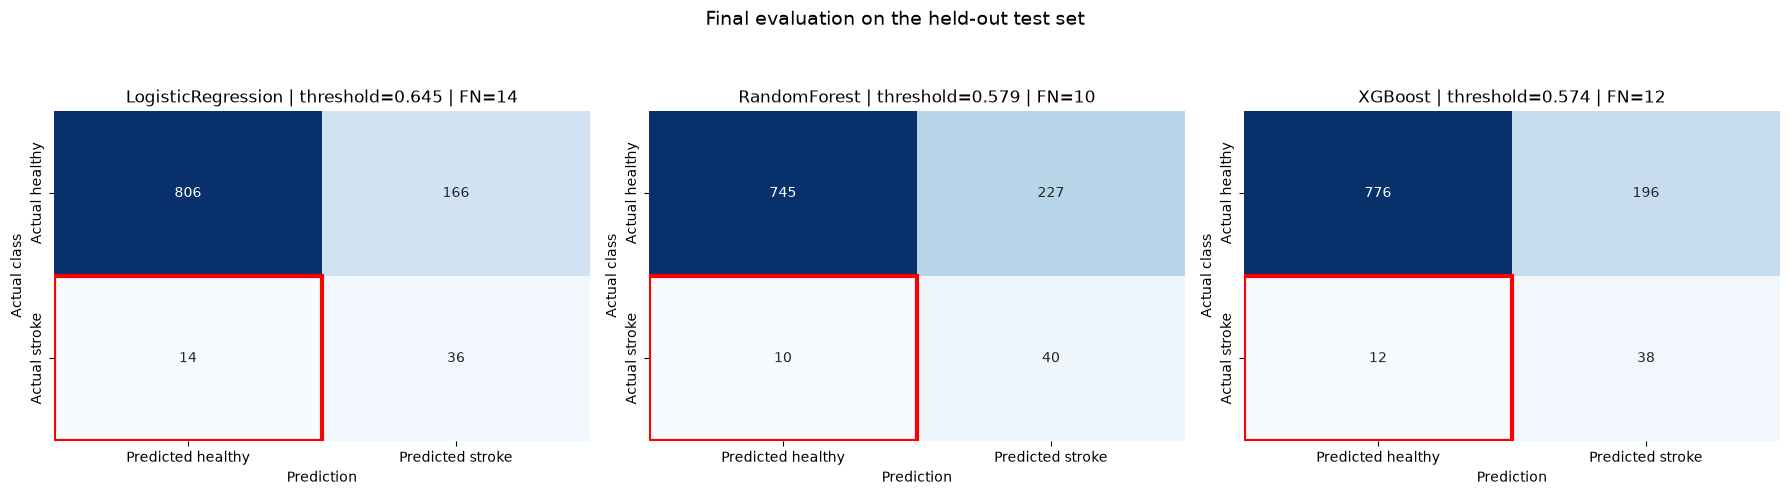
\includegraphics[width=\textwidth]{figures/05_confusion_matrices.png}
    \caption{Matrices de confusion sur le test pour les trois modèles et leurs seuils optimisés sur le train. Les faux négatifs, situés en bas à gauche, sont encadrés en rouge.}
    \label{fig:matrices-confusion}
\end{figure}

\section{Sélection du modèle champion et export}
Le modèle champion est choisi sans consulter les scores du test : la règle appliquée sélectionne le modèle au rappel OOF le plus élevé parmi ceux satisfaisant le plancher de spécificité. Selon l'exécution du notebook, le modèle retenu est la \textbf{Random Forest}, avec un rappel OOF de 0,769 et une spécificité OOF de 0,776 au seuil correspondant. Son rappel test de 0,80 confirme ensuite, à titre d'évaluation indépendante, le résultat de cette sélection.

Le modèle réentraîné sur l'intégralité du jeu d'entraînement et ses métadonnées sont exportés aux emplacements suivants :
\begin{itemize}
    \item Modèle : \path{../data/processed/final_model.joblib} ;
    \item Métadonnées : \path{../data/processed/model_metadata.json}.
\end{itemize}
Les métadonnées conservent notamment le nom du modèle, la règle de sélection, la spécificité minimale et le seuil numérique exact. Pour le modèle exporté, ce seuil vaut :
\[
\texttt{decision\_threshold} = 0.5792571442648802.
\]
La future API FastAPI devra charger le modèle et appliquer cette valeur exacte à la probabilité de la classe AVC, selon la règle \(p \geq \texttt{decision\_threshold}\). Remplacer ce seuil par 0,50 — ou par la valeur d'exemple 0,18 — modifierait le comportement validé et les compromis mesurés. L'ordre des caractéristiques enregistré dans les métadonnées doit également être respecté lors de la construction de l'entrée du modèle.

\section{Portée et limites de l'évaluation}
Cette évaluation confirme la faisabilité d'un réglage de seuil orienté vers le rappel tout en imposant une contrainte explicite sur la spécificité. Elle ne constitue pas une validation clinique du système : la faible précision observée, la variabilité liée à un nombre limité de cas AVC dans le test et les conséquences opérationnelles des faux positifs requièrent une étude complémentaire. Avant tout déploiement, il faudra notamment valider le pipeline complet sur des données externes, vérifier la calibration des probabilités, suivre les performances selon les sous-groupes pertinents et faire approuver le seuil par les responsables cliniques.

\chapter*{Conclusion générale}
\addcontentsline{toc}{chapter}{Conclusion générale}

Ce projet a étudié la faisabilité d'un système de détection précoce des AVC à partir de données fortement déséquilibrées. L'exploration a notamment mis en évidence une association importante entre l'absence de mesure de l'IMC et la prévalence observée de l'AVC : celle-ci atteint 19,90\,\% lorsque l'IMC est manquant, contre 4,26\,\% lorsqu'il est renseigné. Ce constat a motivé la création de l'indicateur \texttt{bmi\_missing}, sans interpréter cette association comme une relation causale ni conclure à lui seul sur le mécanisme de non-réponse.

Le travail de préparation a conservé cette information, plafonné les valeurs extrêmes de l'IMC au lieu d'éliminer les dossiers concernés et séparé le jeu train/test avant l'ajustement des statistiques d'imputation et de standardisation. Les opérations apprises ont ainsi été ajustées sur le train, puis appliquées au test. Le benchmark a comparé plusieurs familles de modèles et stratégies de pondération ou de rééchantillonnage ; l'encapsulation de SMOTE dans un pipeline a permis de limiter son application aux plis d'entraînement pendant la validation croisée. Les modèles arborescents ont par ailleurs été régularisés afin de réduire leur complexité.

L'apport méthodologique central est l'optimisation du seuil à partir de probabilités \textit{out-of-fold} calculées sur le train. Le critère \(F_2\) a privilégié le rappel, tout en maintenant un plancher de spécificité fixé à 0,70 pour encadrer la charge de faux positifs. Ce plancher constitue une contrainte opérationnelle du projet, et non une norme clinique universelle. La règle de sélection, établie sans consulter le test, a retenu la Random Forest. Son seuil est \(0.5792571442648802\) ; sur le test indépendant, elle obtient un rappel de 0,80 et une spécificité de 0,766, avec 10 faux négatifs parmi les 50 cas AVC. La précision de 0,150 et les 227 faux positifs observés montrent cependant que le compromis reste exigeant et doit être évalué avec les équipes cliniques.

Les résultats ne constituent pas une validation médicale ni une preuve de généralisation à d'autres établissements ou populations. Ils dépendent du jeu disponible, et le nombre de cas AVC dans le test reste limité. En outre, dans la version étudiée, les colonnes issues du One-Hot Encoding ont été établies avant le split ; une évolution devra ajuster et sérialiser l'encodeur exclusivement sur le train pour renforcer l'isolation du schéma des catégories. Des validations externes, une analyse de calibration et une étude des performances par sous-groupes sont également nécessaires avant tout usage opérationnel.

\section*{Perspectives}
La prochaine étape consiste à encapsuler le modèle exporté et ses artefacts de prétraitement dans un microservice FastAPI. Des schémas Pydantic pourront valider les champs, les types, les valeurs admissibles et les règles de cohérence des requêtes. Le service devra respecter l'ordre des caractéristiques et le seuil exact conservé dans \texttt{model\_metadata.json}, puis retourner un score et une catégorie d'aide au triage sans se substituer au jugement médical.

Ce microservice pourra ensuite servir d'interface backend à une application Next.js destinée aux urgentistes. La mise en production devra être précédée de tests d'intégration et de sécurité, d'une validation clinique appropriée, ainsi que d'un suivi continu de la calibration, des faux négatifs, de la charge d'alertes et de toute dérive des données.


\clearpage
\phantomsection
\addcontentsline{toc}{chapter}{Bibliographie}
\nocite{*}
\bibliographystyle{plain}
\bibliography{references}

\end{document}
